\documentclass[12pt, letterpaper]{article}
\usepackage{color}
\usepackage{natbib}
\usepackage{parskip}
\usepackage{amsmath}
\usepackage{amssymb}
\usepackage{graphicx}
\usepackage{listings}
\usepackage{setspace}
\usepackage{geometry}
\usepackage{dirtytalk}
\usepackage{subcaption}
\usepackage{indentfirst}
\usepackage{anyfontsize}
\usepackage[utf8]{inputenc}

\parindent=0.5in

\graphicspath{{./imgs/}}

\definecolor{codegray}{rgb}{0.2,0.2,0.2}
\definecolor{codepurple}{rgb}{0.58,0,0.82}
\definecolor{backcolor}{rgb}{0.95,0.95,0.92}

\lstdefinestyle{scheme}
  {backgroundcolor=\color{backcolor},
  commentstyle=\color{blue},
  keywordstyle=\color{magenta},
  numberstyle=\tiny\color{codegray},
  stringstyle=\color{codepurple},
  basicstyle=\footnotesize\ttfamily,
  morekeywords={*},
  breakatwhitespace=false,
  breaklines=true,
  captionpos=t,
  keepspaces=true,
  numbers=left,
  numbersep=5pt,
  showspaces=false,
  showstringspaces=false,
  showtabs=false,
  tabsize=2,
  title=\lstname,
  language=Python
}

\lstset{style=scheme}

\doublespace{}
\title{Discussing the use of reaction diffusion equations for the simulation of physical phenomena}
\author{Simon Abrelat}
\date{\vspace{-5ex}}

\DeclareUnicodeCharacter{2212}{-}
\begin{document}

\large
{\fontsize{12}{14.4}
  {\singlespace{}
  \pagenumbering{gobble}
  \maketitle
  \begin{center}
  \vspace{4mm}
  002129--0004 \\
  \vspace{4mm}
  Math HL IA \\
  \vspace{4mm}
  May 2019 \\
  \vspace{4mm}
  Words: \\
  \end{center}
  }
}
\newpage

\pagenumbering{arabic}
\begin{abstract}
  This is the thing working good \citep{turing}, here is another example \citep*{grayscott}
\end{abstract}

\newpage
\tableofcontents
\newpage 

\section{Introduction}

\section{Calculus}
Reaction diffusion relies on multi-variable calculus, from the partial derivative to the Laplacian 
operator that governs diffusion. Multi is a natural extension of calculus where instead of 
focusing on the accumulation and change on 1 axis, that being y, it is possible to do in to any
number of dimensions. This means that if your function has more than 1 input, like for 3D functions, you would
have a new arsenal of tools and methods to analyse your equations. The most simple being the limit which
fundamentally operates the same as in the normal case. If there is a hole in the function but otherwise is
continuous, it would \say{fill in} that hole, and if there is a jump discontinuity the limit is defined some
certain directions but the limit itself is undefined. Once again using the concept of limits we can get the
integral and derivative as in normal calculus; however for this application we will be primarily focusing on
partial derivatives and other related operations. Instead derivatives in in multivariate partial derivatives are used. These are computed in a similar form to derivatives but the input that is not differentiated is
treated as a constant. For use in the reaction equations the partial differential equations behave in asimilar way to differential equations but rely on more inputs but are still the rate of change in a given 
input over a function.

\begin{gather}
  \frac{\partial f}{\partial x} = \partial_x{f} = \lim_{h \to 0} \frac{f(x+h, y) − f(x,y)}{h}
  \label{eq:partX}
\end{gather}
\begin{gather}
  \frac{\partial f}{\partial y} = \partial_y{f} = \lim_{h \to 0} \frac{f(x, y + h) − f(z,y)}{h}
  \label{eq:partY}
\end{gather}

\begin{center}
 Example problem
 \begin{gather*}
  f(x, y) = xy^2 + x \\
  \partial_x f(x,y) = y^2 + 1 \\
  \partial_y f(x,y) = 2xy
 \end{gather*}
\end{center}

\begin{figure}[t]
  \centering
  \begin{subfigure}[b]{.75\linewidth}
    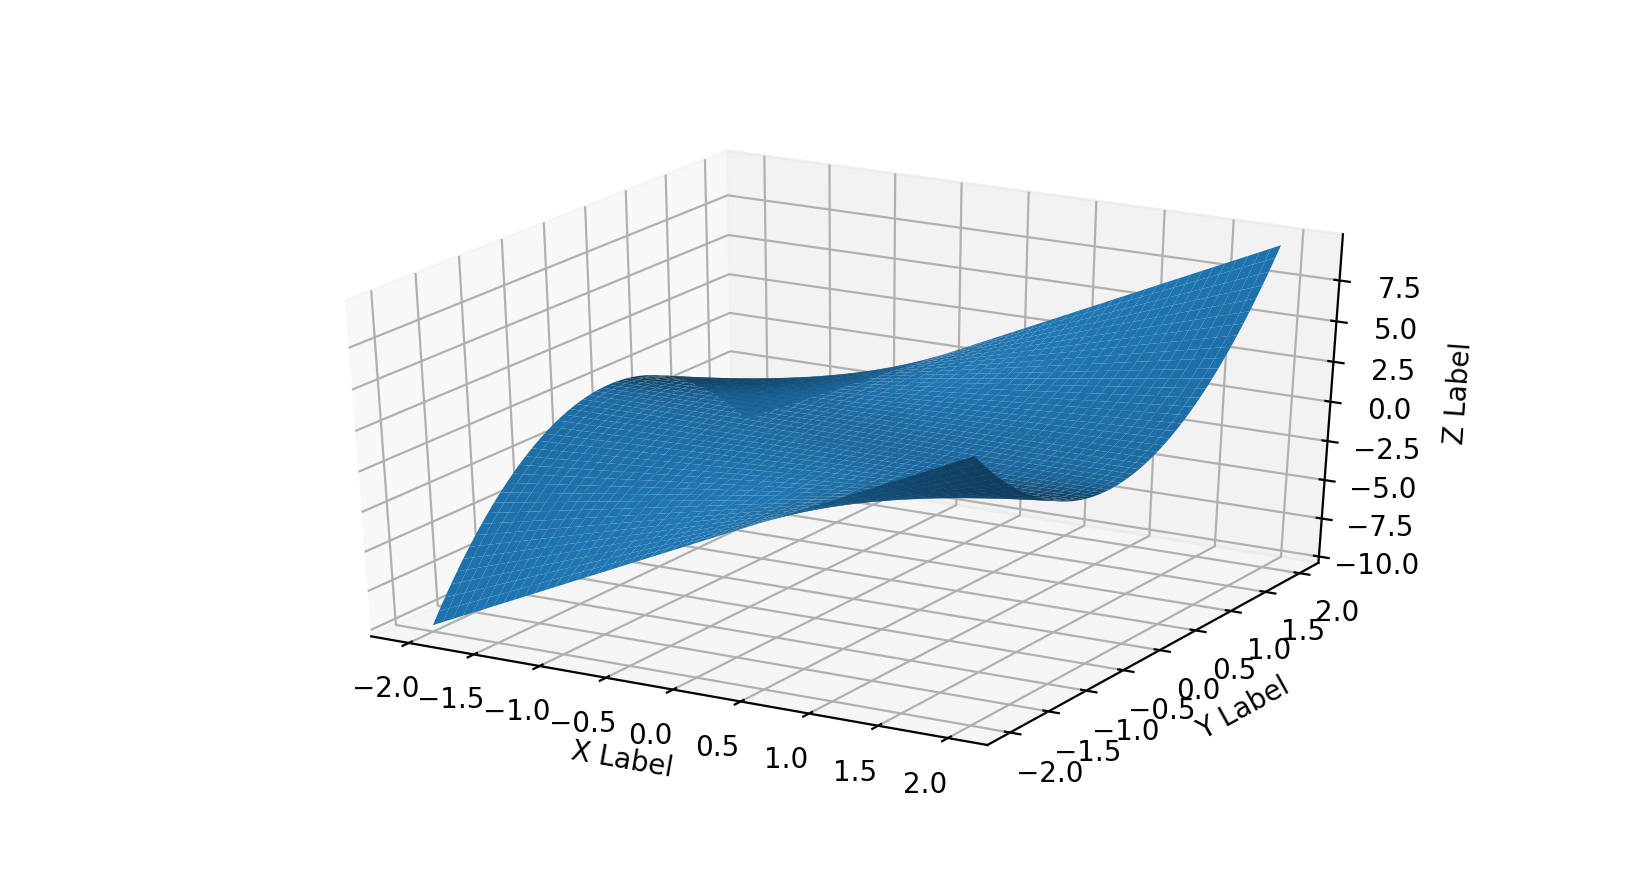
\includegraphics[width=\linewidth]{multifn}
    \caption{$f(x,y) = xy^2 + x$}
  \end{subfigure}

  \begin{subfigure}[b]{.45\linewidth}
    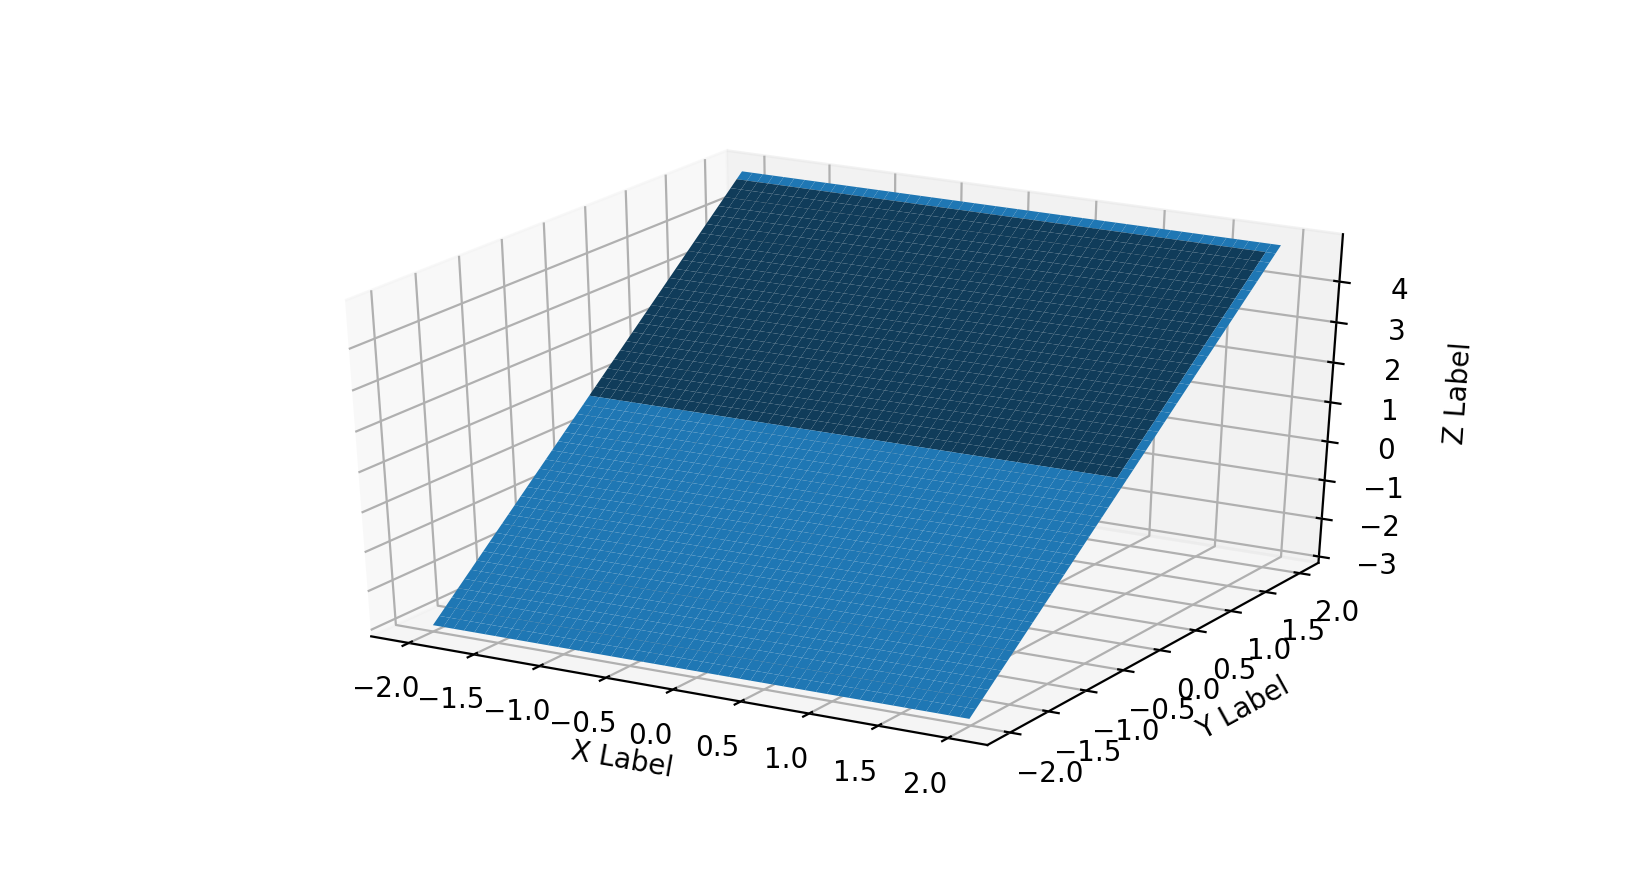
\includegraphics[width=\linewidth]{partDervX}
    \caption{$\partial_x f(x,y) = y^2 + 1$}
  \end{subfigure}
  \begin{subfigure}[b]{.45\linewidth}
    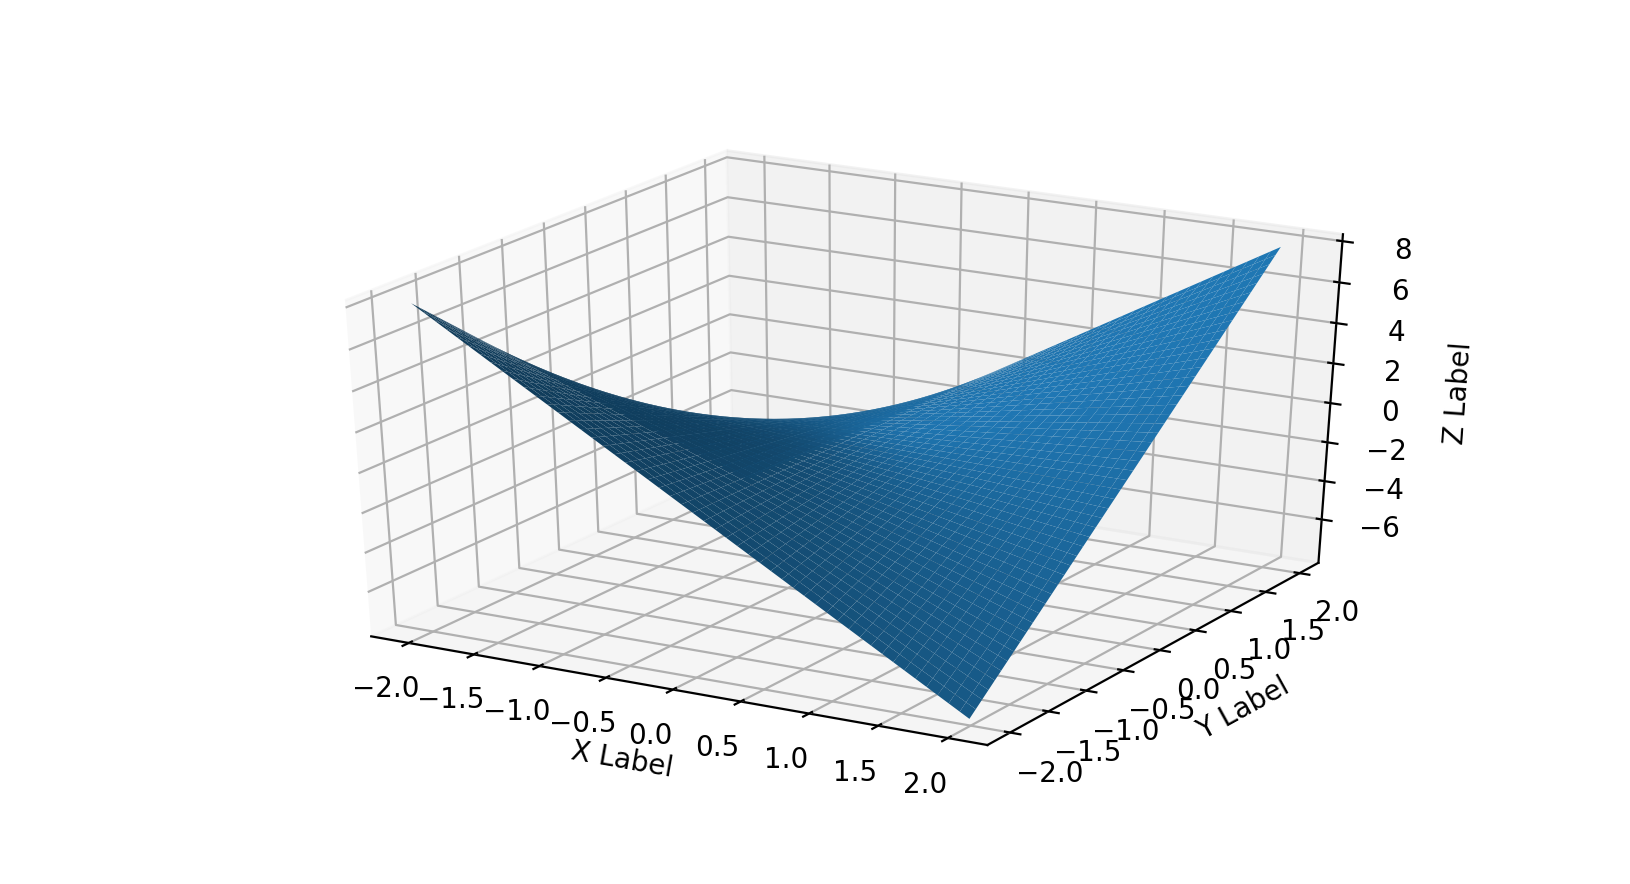
\includegraphics[width=\linewidth]{partDervY}
    \caption{$\partial_y f(x,y) = 2xy$}
  \end{subfigure}
  \caption{Example functions}
\end{figure}

\newpage{}
Then there are directional derivatives which are similar to the partial derivatives, but instead of being in a component direction like along the x  or y direction it would be in the direction of the vector $\vec{u}$
with components $ <a, b> $. These derivate can be done in any number of dimensions (\ref{eq:NDirectional})
but for reaction diffusion formulas shown 2D cases (\ref{eq:2Directional}) matter more.

\begin{equation}
  D_u f = \lim_{h \to 0} \frac{f(x + ha, y+ hb) − f(x, y)}{h}
  \label{eq:2Directional}
\end{equation}
\begin{equation}
  D_u{f(\vec{x})} = \lim_{h \to 0} \frac{f(\vec{x} + hu) − f(\vec{x})}{h}
  \label{eq:NDirectional}
\end{equation}
The directional derivative can also be written as a dot products
\begin{gather*}
\begin{aligned}
  D_u f(x,y) &= a\partial_x f + b\partial_y f \\
             &= <\partial_x f, \partial_y f> * <a, b> \\
             &= <\partial_x f, \partial_y f> * u \\
             &= \nabla f(x,y) * u 
\end{aligned}
\end{gather*}

This $\nabla$, or nabla, is the sign for the grad operator read \say{del f} This represents a vector of all
of the partial derivatives that are possible in a function called the gradient. For example in $g(x, y, z)$,
grad g= the partial derivative of g in respect to x, y, and z. This gradient should the direction of the
fastest increase of the function. So if we had a map of a mountain range the gradient of the map from a
point would be the fastest way to get to the top of the nearest mountain but not necessarily the highest
mountain. The gradient is often used for optimization problems since it can go \say{the highest} or most
optimal local  point in a function of any number of variables. A common abuse of notation is to set $\nabla$
to a value (\ref{eq:nabla})
\begin{equation}
  \nabla = <\frac{\partial}{\partial x}, \frac{\partial}{\partial y}, \frac{\partial}{\partial z}>
  \label{eq:nabla}
\end{equation}

So the notation for the gradient makes since because you would be treating the function f as a scalar and
multiplying it to the $\nabla$ vector. This abuse of notation since it would also make sense for the
divergence of a vector field. For a vector field the function F (\ref{eq:vectorFn}) would be a vector function
where you could dot product of F and $\nabla$ (\ref{eq:div})

\begin{figure}[!b]
  \centering
  \begin{subfigure}[b]{.45\linewidth}
    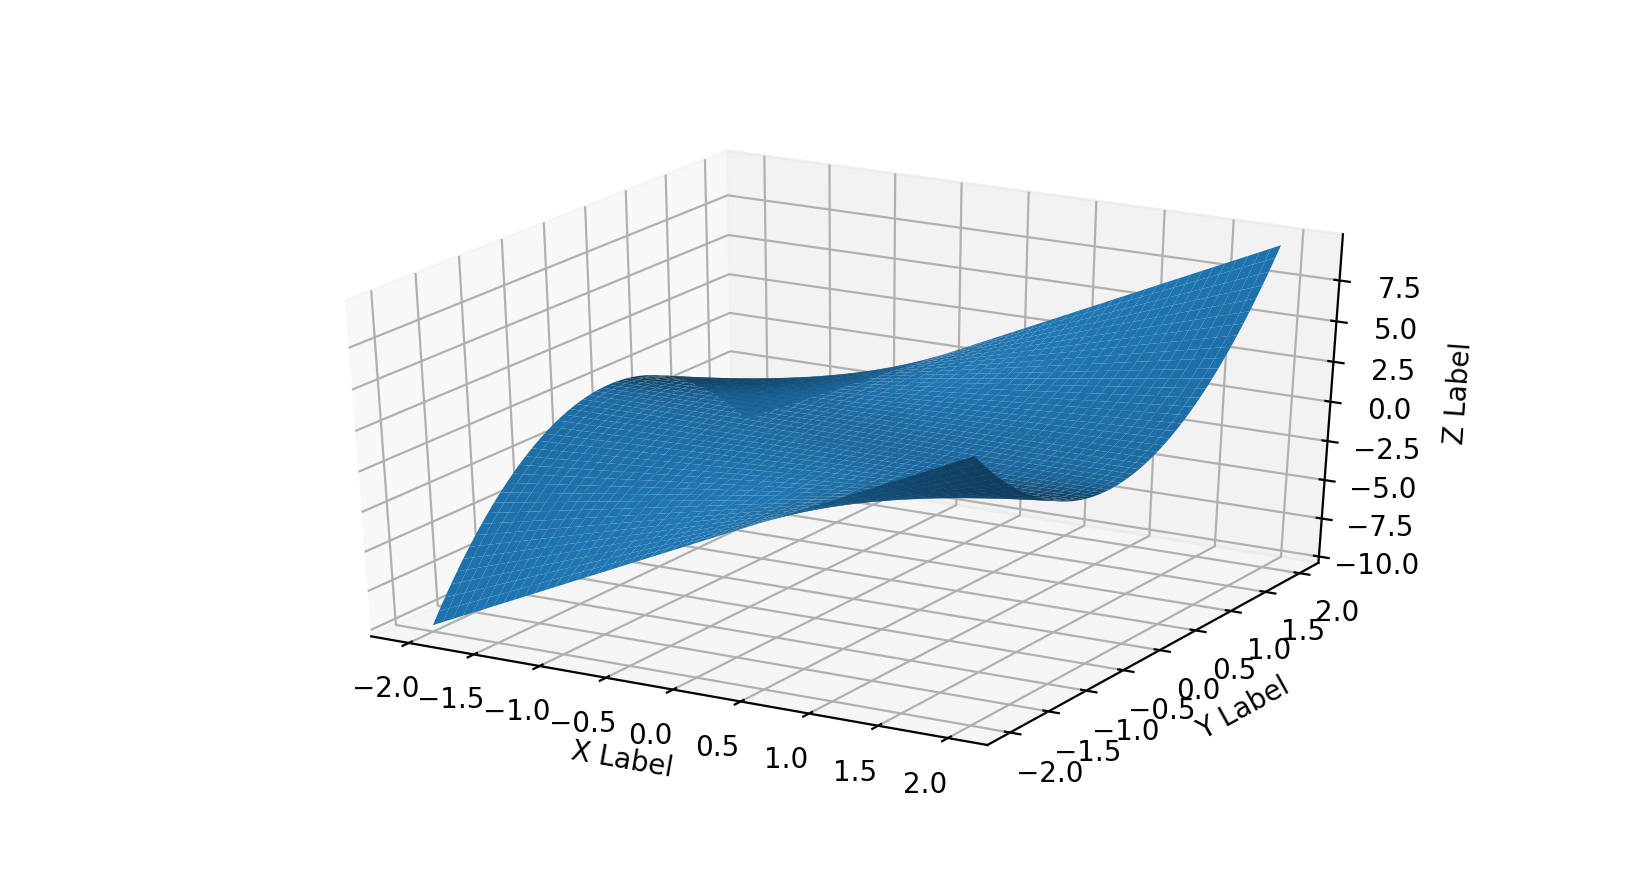
\includegraphics[width=\linewidth]{multifn}
    \caption{$f(x,y) = xy^2 + x$}
  \end{subfigure}
  \begin{subfigure}[b]{.5\linewidth}
    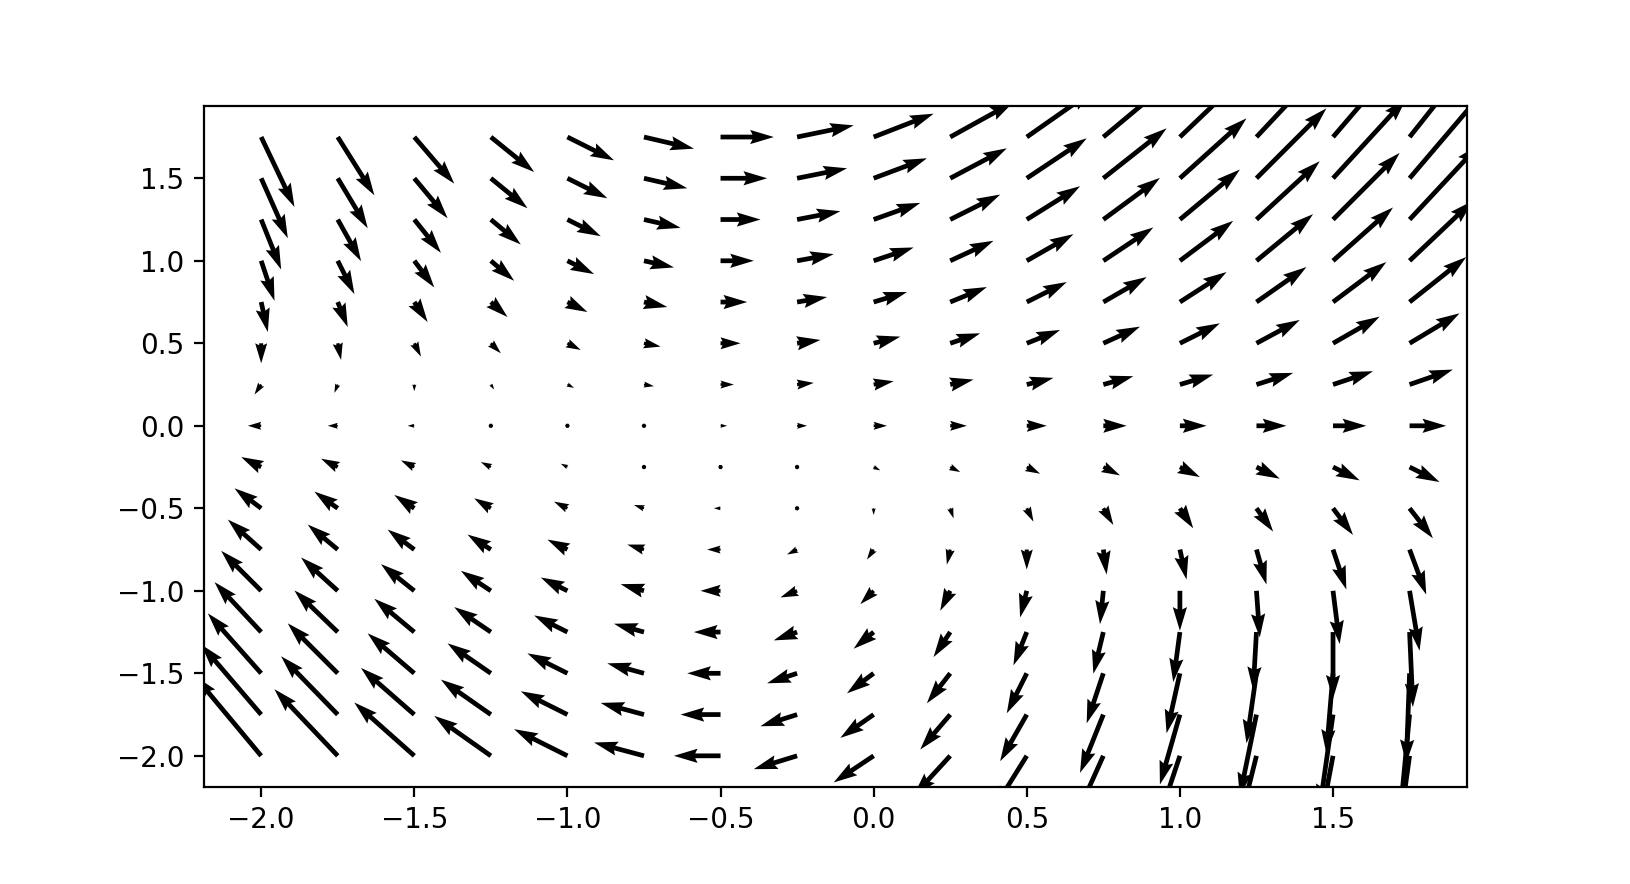
\includegraphics[width=\linewidth]{gradient}
    \caption{the gradient vector field: $\nabla * f(x,y)$}
  \end{subfigure}
\end{figure}

\begin{equation}
  \bold{F} = P\hat{\imath} + Q\hat{\jmath} + R\hat{k} \\
  \label{eq:vectorFn}
\end{equation}
\begin{equation}
  div \bold{F} = \nabla * \bold{F} = \frac{\partial P}{\partial x} + \frac{\partial Q}{\partial y} +
 \frac{\partial R}{\partial z}
  \label{eq:div}
\end{equation}

\newpage
One can picture a vector field as being a model of fluid flow, where the vector at a point would be the
velocity of the fluid. Given this analogy, the divergence if the fluid is incompressible then the amount of
fluid that emanates from a point. In a vector field that would represented by all of the arrows pointing away
from a point and the arrows get larger around a point then the divergence $>$ 0 and if the arrows are smaller
or point inwards than the divergence $<$ 0. Both of these tools are useful but when applied together become
what is needed for the diffusion part of reaction diffusion that being the laplacian. The laplacian is the
divergence of the gradient of a function.

\begin{center}
Laplacian = $\nabla * (\nabla f) = \nabla^2 f = \frac{\partial^2 f}{\partial x^2} + \frac{\partial^2
f}{\partial y^2} \frac{\partial^2 f}{\partial z^2} = \sum_{i=1}^{n} \frac{\partial^2 f}{\partial x_i^2}$ \quad
$\nabla^2 = \nabla * \nabla$
\end{center}

This is called the Laplace operator or the Laplacian of a field because of its relation to Laplace's
Equation which has similarities to the heat transfer equation for diffusion. The reason that when put in
PDEs they exhibit this diffusion or spreading properly is due to their relation to the second derivative in
normal calculus. They identify local maxima and minima but in normal calculus where the second derivative is
0 in both cases the laplacian is highly positive in minima and highly negative in maxima. In the case of
PDEs, that would mean that the values would \say{move away} from maxima and \say{fill in} minima which exactly
describes osmosis and other diffusion systems.

\begin{equation}
  \nabla^2 \bold{F} = \frac{\partial^2 f}{\partial x^2} + \frac{\partial^2 f}{\partial y^2} +
  \frac{\partial^2 f}{\partial z^2} = 0
  \label{eq:laplaces}
\end{equation}

Equations that satisfies Laplace's Equation (\ref{eq:laplaces}) are called harmonic functions where at all points the value of
the laplacian = 0 

\section{Diffusion}

Diffusion is the spread of things from high to low densities. A simple example would be heat or osmosis in 
cells. In general this is seen as spreading out, like there is diffuse light. The mathematical way this is
described is through a partial differential equation using the Laplace operator, $ \nabla^2 $.

\begin{equation}
  \frac{\partial u}{\partial t} = \alpha \nabla^2 u
  \label{eq:heatDiff}
\end{equation}

\begin{equation}
  \frac{\partial u}{\partial t} = \alpha (\frac{\partial^2 u}{\partial x^2} + \frac{\partial^2 u}{\partial
  y^2} + \frac{\partial^2 u}{\partial z^2})
  \label{eq:heatDiff3}
\end{equation}

This equation~\ref{eq:heatDiff} is a rather simple partial differential equation that has $u(x, y, z)$ 
to determine the heat and $\alpha$ as the coefficient of thermal diffusivity. Because of the Laplace
operator, the equation does not need to show its inputs which also allows for a N-dimensional continuation.
In 3 dimensions this equation can be expanded into equation~\ref{eq:heatDiff3}.

\begin{figure}[h]
\label{fig:progression}
  \centering
  \caption{Heat Diffusion Progression}
  \begin{subfigure}[b]{.21\linewidth}
    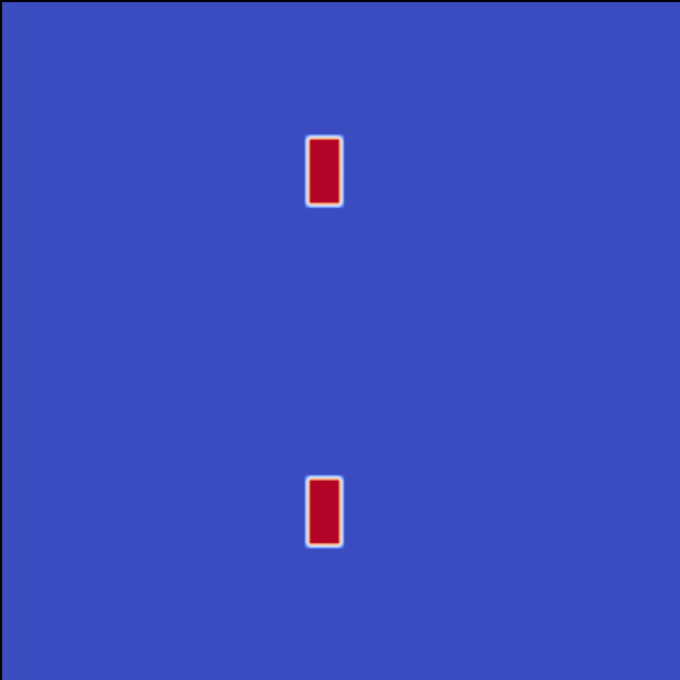
\includegraphics[width=\linewidth]{HeatProgression/diffusion0}
    \caption{$n=0$}
  \end{subfigure}
  \begin{subfigure}[b]{.21\linewidth}
    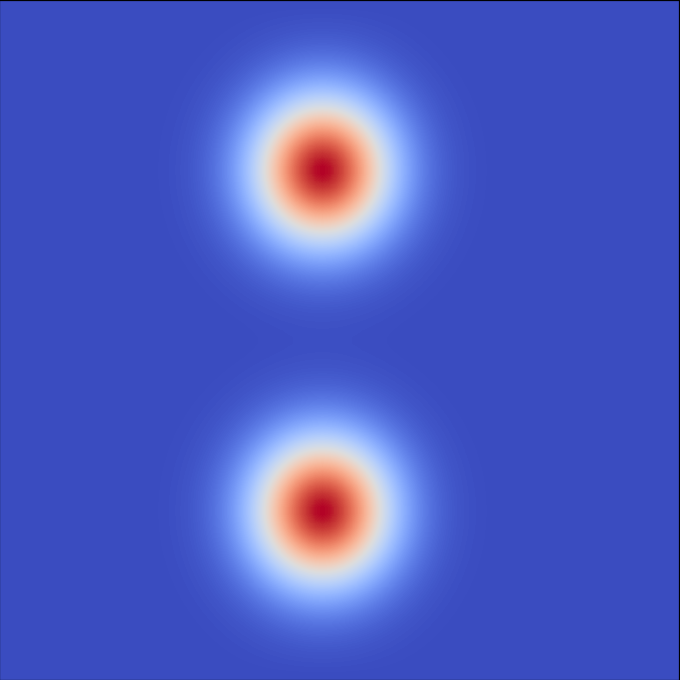
\includegraphics[width=\linewidth]{HeatProgression/diffusion1000}
    \caption{$n=1000$}
  \end{subfigure}
  \begin{subfigure}[b]{.21\linewidth}
    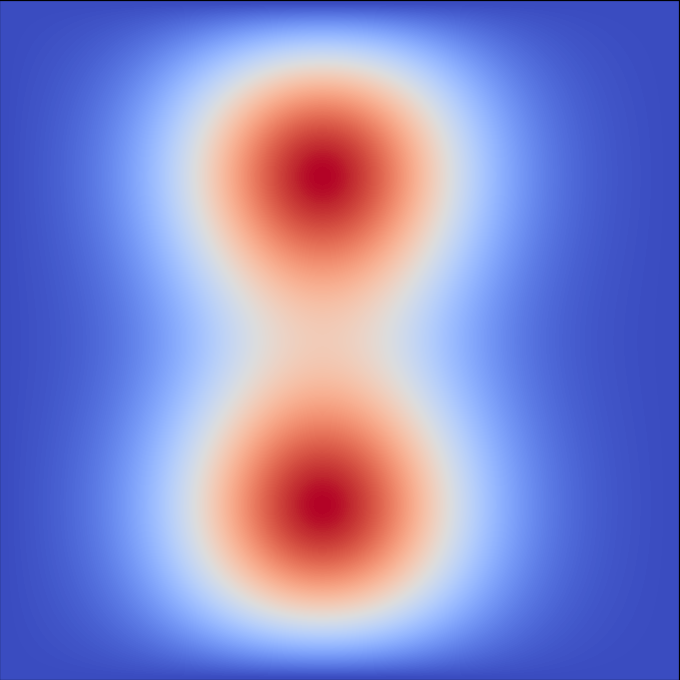
\includegraphics[width=\linewidth]{HeatProgression/diffusion5000}
    \caption{$n=5000$}
  \end{subfigure}
  \begin{subfigure}[b]{.21\linewidth}
    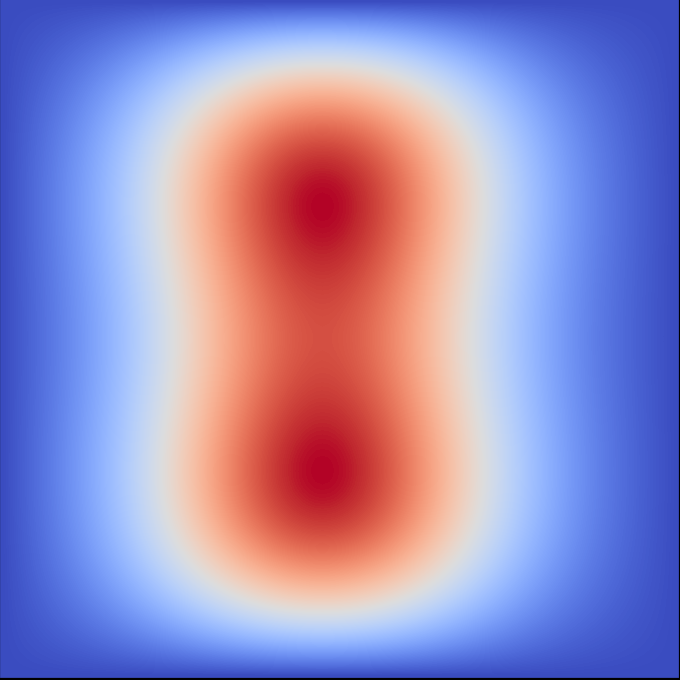
\includegraphics[width=\linewidth]{HeatProgression/diffusion8000}
    \caption{$n=8000$}
  \end{subfigure}
\end{figure}

In this case, (Fig.~\ref{fig:progression}) is progression from 2 point heat sources that spread out
and then eventually merge into a single blob that then continues to spread making the entire plane warmer.

The heat diffusion equation (\ref{eq:heatDiff}) uses the laplacian which \say{pushes} the local maxima down 
and the local minima up. Later in the reaction diffusion equations, the laplacian is used to give the
equations properties based off their location and physical proximity to other elements. This diffusion
component gives reaction diffusion equations their interesting properties since previously converging
reactionary systems remain in this possibly unstable equilibrium. The reason for this is that the reactions,
spreading due to diffusion, would encounter more fuel as they go until they eventually run out then generating
some homeostasis.

\section{Reaction}
In contrast to diffusion equations there are significant differences between different reaction systems.
They are called \say{reaction systems} since they typically contain multiple ordinary or partial 
differential equations. Were diffusion equations usually have only one variable, reaction systems are often
multi variable. There are so many different examples of reaction system, but the SIR and Lotka-Volterra Model.

\begin{equation}\label{eq:SIR}
  \begin{split}
    &\frac{dS}{dt} = -\beta s(t) i(t) \\
    &\frac{dI}{dt} = -\beta s(t) i(t) - \kappa r(t) \\
    &\frac{dR}{dt} = \kappa r(t)
  \end{split}
\end{equation}

The SIR model (\ref{eq:SIR}), or Susceptible-Infected-Recovered Model, is an computational epidemiology and
serves as the core of other more advanced models. In this system, $\kappa$ represents the days until
recovery, and $\beta$ represents the number of days to be in contact required to spread the disease. This
model is intuitive. The recovered is the number of infected times the rate of recovery. The susceptible
population is the number of people times the number of infect and the rate of spread. Finally, the infected
are the ones that are left over. 

\section{Reaction Diffusion}
\bibliographystyle{apa}
\bibliography{EE}
\newpage
\section{Appendix}
{\lstinputlisting[language=Python, caption=Surface]{code/surface.py}
 \label{alg:surfaceCode}}
{\lstinputlisting[language=Python, caption=Gradient]{code/gradient.py}
 \label{alg:gradientCode}}
{\lstinputlisting[language=Python, caption=Diffusion]{code/diffusion.py}
 \label{app:diffusionCode}}
{\lstinputlisting[language=Python, caption={Lotka-Volterra}]{code/lotkaVolterra.py}
 \label{app:lotkaVolterraCode}}
{\lstinputlisting[language=Python, caption=SIR]{code/SIR.py}
 \label{app:SIRCode}}
\end{document}
